\documentclass[main.tex]{subfiles}
\ProvidesPackage{preamble}

\usepackage[nottoc]{tocbibind}
\usepackage[english]{babel}
\usepackage[utf8]{inputenc}
\usepackage[table]{xcolor}
\usepackage[nohead, nomarginpar, margin=1in, foot=.25in]{geometry}
\usepackage{tabularx}
\usepackage{graphicx}
\usepackage{float}
\usepackage[english]{babel}
\usepackage{paralist}
\usepackage{datetime}
\usepackage{afterpage}

\begin{document}

\section{Background and Competitors}
As a result of our initial competitor analysis, we may group the competing software into two categories. For a comprehensive list of available backtesters please see \cite{listofbacktesters}. The first consists of various third-party trading software, such as Fidelity \cite{Fidelity}, MetaTrader \cite{MetaTrader} and NinjaTrader \cite{NinjaTrader} that offer backtesting features as well. Services in this category include features such as buying and selling of financial assets, prediction of future prices and storing and managing of users' money. Although it may be beneficial to consider some features related to real time trading, these would only be part of a future development process, and are not in the scope of our prototype.

The second category consists of pieces of software that do not offer trading as a service, and solely focus on backtesting. Thus, for now, we shall only consider the feature set provided by the second category. In the following paragraphs we will consider some of the design decisions made by competing software, together with the brief analysis and conclusion on each feature.

\subsection{Portfolio Visualizer}
Our main competitor of the second category is an online backtesting tool named Portfolio Visualizer\cite{portfoliovis}. During the inception phase of development we heavily relied on this website for writing the requirement analysis. Let us now briefly dissect what it has to offer. 

Upon opening the website we are greeted with a brief description of the domain, together with the following input form:

\begin{figure}[H]
   \centering
   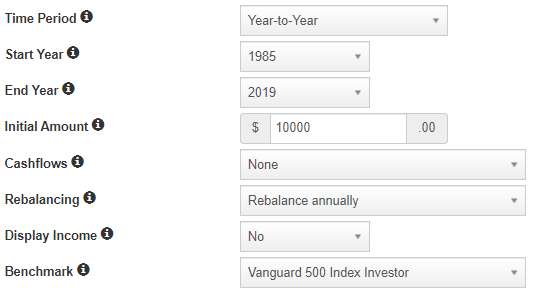
\includegraphics[scale=0.8]{02Background/02Pictures/portfolio_visualizer_input_1.png}
   \caption{Portfolio Visualizer - Input (source: https://www.portfoliovisualizer.com/)}
\end{figure}

As we can already see, the key elements of portfolio analysis are provided. Considering the functionality of our prototype as a baseline (that is testing an allocation of assets with a fixed initial investment on a fixed time period), we see that in addition users are able to do the following set of features:

\begin{itemize}
  \item Set the endpoints of the investment period, up to months.
  \item Set the initial investment. 
  \item Specify a regular cashflow and its frequency.
  \item Select a rebalancing strategy.
  \item Select a benchmark strategy for comparison.
  \item Compare multiple strategies at the same time.
  \item Adjust to inflation.
  \item Select from a set of lazy portfolios.
  \item Calculate additional metrics. 
  \item Export the results to PDF, Excel, or save link. 
\end{itemize}

At first it may seem as if Portfolio Visualizer meets all the requirements needed for a financial backtester, and indeed our main criticism is regarding the UI, responsiveness and user experience, and is a result of the initial user testing. 

The UI design is simplistic and has a non-commercial, bare-bones look, and although this was appreciated while testing the system it certainly does not improve the user experience. The input, mostly using dropdown menus is straightforward to use, except for the selection of Assets, which we will discuss briefly at the end of this section.

Moreover, users will want to fine-tune their investment strategies, by changing their allocations frequently. The only means to do this using Portfolio Visualizer is to scroll to the top, change the input and rerun the entire simulation. Our goal is to design a more responsive and dynamic system, to ease this procedure. 

The website also has user accounts, however little to no data is associated with a user's profile, which further decreases the overall user experience. Finally, as a last remark, which holds for most of the backtesting tools we have tried, the website is heavily US biased, and so the selection of asset classes is limited. Furthermore, we have no means of changing the currency, which would also be an important feature for a product accessible through the web (and therefore available to users from all over the globe).

\subsection{Other Competing Software}

The rest of the alternatives are of a significantly lower quality. In the remaining parts of this section we will briefly consider a few design decisions made by these websites.

\subsubsection*{Tree-like Asset Selection}

One challenging aspect of designing such a system is the following: 

\begin{quote}
    What is the most intuitive way for selecting a portfolio item? 
\end{quote}

Where a portfolio item could be: an equity, ETF index, a commodity, bond or stock. Within these classes we have more options to choose from. Many backtesters opted for a search bar, which is a sensible approach, but poor in practice. Many portfolio items are named similarly, and for a new user it is a barrier, as they might not know what is available. 

One of the better option is what ETFReplay \cite{etfreplay} has implemented, which is a tree-like selection form, shown below. 

\begin{figure}[H]
   \centering
   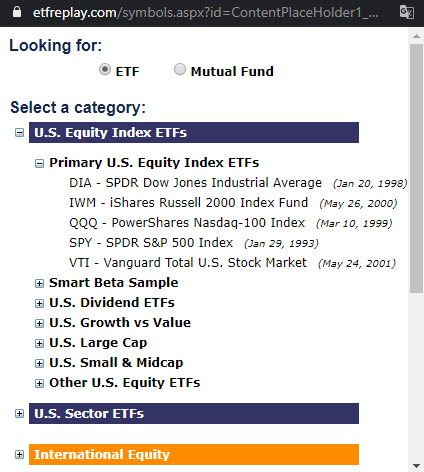
\includegraphics[scale=0.7]{02Background/02Pictures/etfreplay.png}
   \caption{ETFReplay - Tree-like Structure (source: https://www.etfreplay.com/)}
\end{figure}

We feel this was the most intuitive to use, and will thus pursue a similar approach. The only potential issue associated with this is that it opens in a new window, which we would prefer to avoid.

\subsubsection*{Tiles}

It may be worth briefly discussing an example of a backtester with a good layout design. We found the simplistic and tiled design of Backtest Curvo \cite{backtestcurvo} a good choice as it gives the website an overall modern and fresh look, whereas most backtesters looked old and out of date. Our goal is to achieve a layout similar to this. For a further analysis on design decisions, please see section 4 of this report.

\subsubsection*{Simple Logic}

In our whitepaper, we briefly discussed implementing a simple scripting language allowing users to simulate dynamic trading strategies \cite{WP}. As mentioned, this would not be in the scope of the course, but for inspiration we can have a look at the approach of Stockbacktest \cite{stockbacktest}.

\begin{figure}[H]
   \centering
   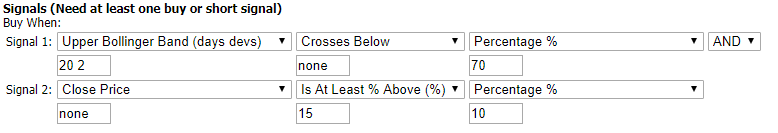
\includegraphics[scale=0.7]{02Background/02Pictures/stockbacktest.png}
   \caption{Stockbacktest - Simple Logic (source: http://stockbacktest.com/)}
\end{figure}

Although not intuitive at all, given its presentation, it shows this feature is also possible. We believe that after nailing down how exactly the user would create the rules, this would be a straightforward task, as the calculations involved are not more complicated than in the static case. As mentioned above, this is something we would like to implement in the future.

\subsection{Summary}
\label{reliability}

As we initially tested the competing software during the inception phase of development, we were left with three key observations. These were the following:

\begin{itemize}
    \item Transparency: Many of the testers' webpages did not give the impression of being operated by a reputable businesses. In the worst case, they gave the impression of being untransparent or untrustworthy (misspelt words, advertisements with questionable subject matter), which is something we should avoid.
    \item Learning Curve: After getting to know our target audience we concluded that most seem willing to learn how to use a complex system if it is worth it.
    \item Design of the UI: It was easy to tell which backtesters are still getting updated, by looking at their design. We should aim at looking fresh. In addition, some backtesters offered so many features that every corner of their UI was packed with information, this is something we should also avoid doing.
\end{itemize}

The analysis was conducted informally with the help of colleagues studying or involved in finance. This allowed us to develop a more neutral and accurate impression, despite the subjective nature of the observations. Having analysed the competing software, we are now better suited to determine the requirements of our system. 

\end{document}
